\chapter{Architectural design}

\section{Overview}
We have chosen to use a top-down approach, so we will start from a higher level of architectural design view and then we will analyse the system deeper.

We have chosen a four-tier architecture in order to keep a logical separation among data level, business level, communication level and client level.

%\begin{table}
\begin{center}
\begin{tabular}{cc}
\toprule
\textbf{Tier}	&	\textbf{Layer}				\\
Client		&	Terminal/Browser				\\
Web		&	\multirow{2}*{Application Server}	\\
Business	&							\\
Data	&	DBMS							\\
\bottomrule
\end{tabular}
%\caption{Architectural tiers}
\end{center}
%\end{table}

\begin{description}
\item[Client Tier] is the level used by the end user and it is located in the terminal mobile app or in the web browser:
\item[Web Tier] is the level that receives communication requests from client and communicates with the Business Tier to formulate responses. It is located in the application server;
\item[Business Tier] is the logical applicative level of the software. It analyses data received from the Data Tier and it provides info's to the Web Tier. It is located in the application server;
\item[Data Tier] is the \emph{Model} in the \emph{Model-View-Controller} pattern and it communicates with the Business Tier. It contains all the software data and is located in a DBMS.
\end{description}

%%%%%%%%%%%%%%%%%%%%%%%%%%%%%%%%%%%%%%%%

\section{High level components and their interactions}
\label{sec:architecture}
\begin{figure}
\centering
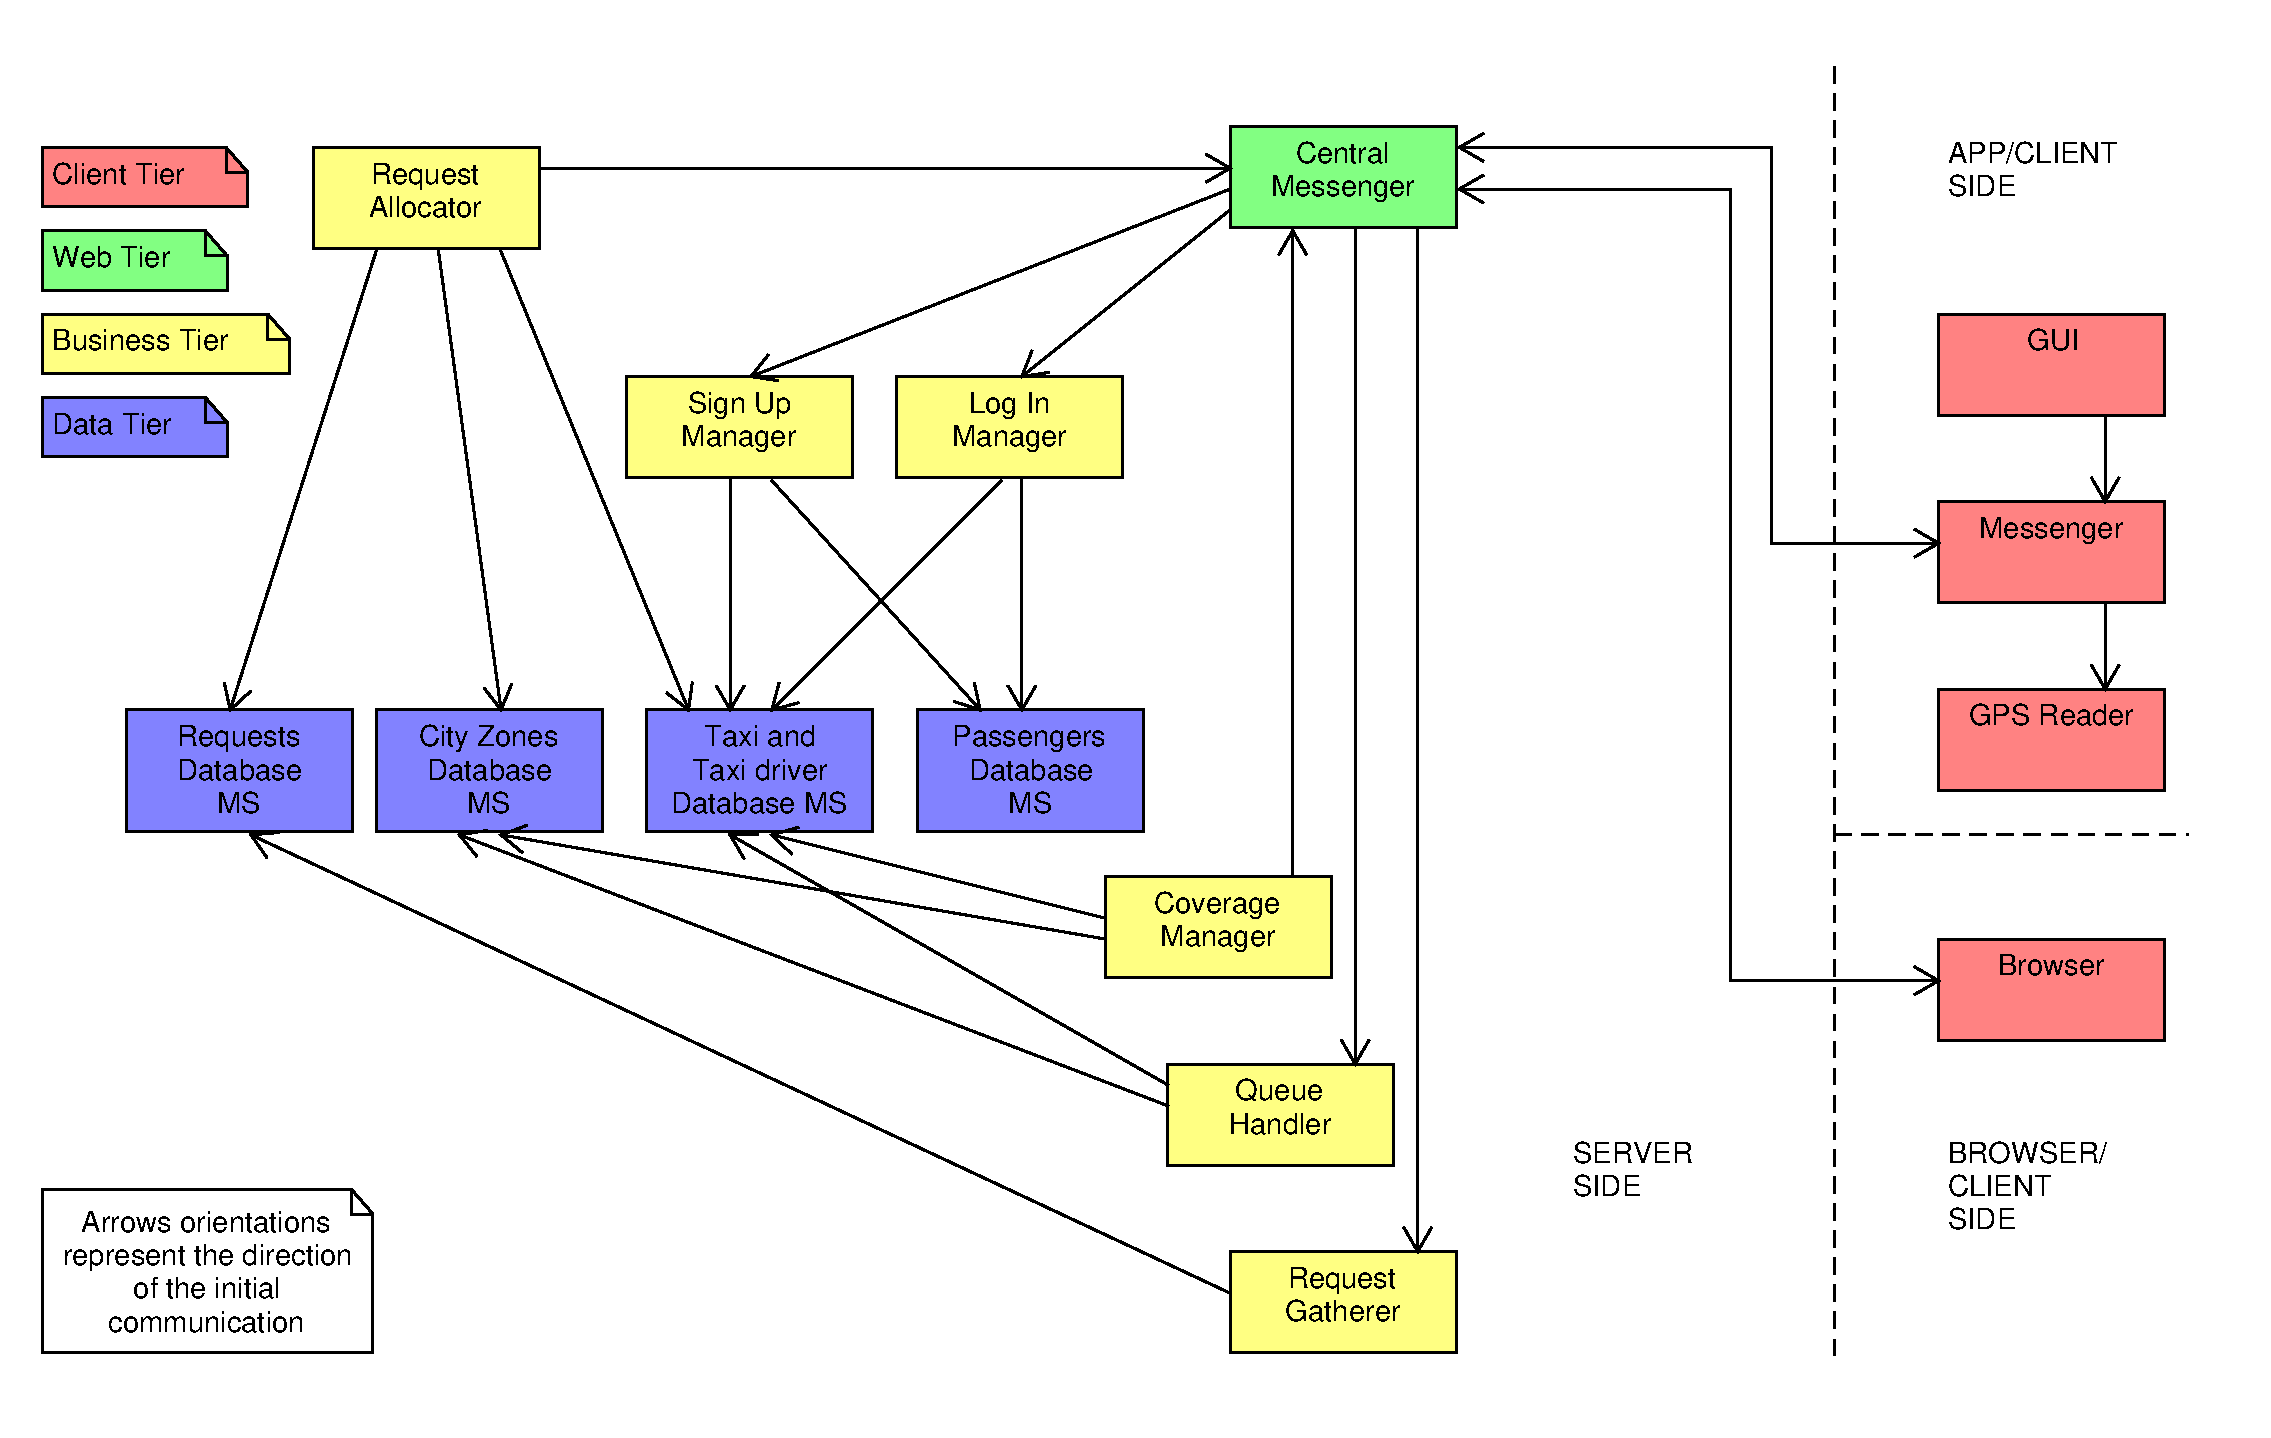
\includegraphics[width=\textwidth]{tex-images/interactions}
\caption{The different architectural components and their interaction}
\end{figure}

For each tier, we have identified a number of high-level architectural components.
\subsection{Client Tier}
\begin{description}
\item[Graphical User Interface] It is the graphical user interface of the mobile application;
\item[GPS Reader] It reads GPS information from the API's of the operative system;
\item[Messenger] It sends and receives messages from Web Tier Central Messenger and handles every message and operation of the Client Tier, in fact it communicates with GPS Reader and GUI;
\item[Browser] It communicates with Web Tier Central Messenger and it represent the User Interface alternative to mobile app.
\end{description}

\subsection{Web Tier}
\begin{description}
\item[Central Messenger] It sends and receives messages from Client Tier and it handles every message and operation among Business Tier components. It also elaborates and sends pages to the Browser;
\end{description}

\subsection{Business Tier}
\begin{description}
\item[Sign Up Manager] It manages the registration function and it operates with the Taxi and Taxi driver DBMS and the Passenger DBMS;
\item[Log In Manager] It manages the Log In function and it operates with the Taxi and Taxi driver DBMS and the Passenger DBMS;
\item[Coverage Manager] It controls and manages continuously the coverage of taxi in the city. It operates with  the Taxi and Taxi driver DBMS and the City Zones DBMS;
\item[Request Gatherer] It collects the requests and reservations and it writes them in the Requests DB;
\item[Request Allocator] It reads from the Requests DB and it allocates requests to taxi drivers. So it also operates with Taxi and Taxi driver DBMS and City Zones DBMS;
\item[Queue Handler] It manages the allocation of taxi drivers in the correct city zone queue. It operates with Taxi and Taxi driver DBMS and City Zones DBMS.
\end{description}

\subsection{Data Tier}
\begin{description}
\item[Requests DBMS] It's the database that contains all reservation and request information:
\item[City Zones DBMS] It's the database that contains all zones information and queues;
\item[Taxi and Taxi driver DBMS] It's the database that contains all taxi drivers information;
\item[Passenger DBMS] It's the database that contains the registered passengers information.
\end{description}

%%%%%%%%%%%%%%%%%%%%%%%%%%%%%%%%%%%%%%%%

\section{Lower level modules view}
After the initial architectural structure was in place, the analysis was refined to identify, for each component, several lower-level modules that compose it.

\subsection{Client Tier}
\subsubsection{Central Messenger}
\begin{itemize}
\item A module that interfaces with GUI;
\item A module that interfaces with GPS Reader;
\item A module that interfaces with Server Central Messenger;
\item A module that handles and forwards messages to modules.
\end{itemize}

\subsubsection{GPS Reader}
\begin{itemize}
\item A module that interfaces with Central Messenger in order to receive requests and send information;
\item A module that reads GPS information from Mobile APIs.
\end{itemize}

\subsubsection{Graphical User Interface}
\begin{itemize}
\item A module that interfaces with Central Messenger in order to receive and send messages;
\item A module that shows navigation pages.
\end{itemize}

\subsection{Web Tier}
\subsubsection{Central Messenger}
\begin{itemize}
\item A module that interfaces with Queue handler;
\item A module that interfaces with Request Allocator;
\item A module that interfaces with Request Gatherer;
\item A module that interfaces with Coverage Manager;
\item A module that interfaces with Sign Up/Log In manager;
\item A module that interfaces with Client Central Messenger;
\item A module that interfaces with Client Browser;
\item A module that handles and forward messages throw modules.
\end{itemize}


\subsection{Business Tier}
\subsubsection{Sign Up Manager}
\begin{itemize}
\item A \emph{Communication module} that interfaces with Central Messenger;
\item An \emph{Analysis module} that, reading form \emph{Data module}, analyses the correctness of data and it eventually confirms or rejects;
\item A \emph{Data module} that stores data in the correct database and read needed information.
\end{itemize}

\subsubsection{Log In Manager}
\begin{itemize}
\item A \emph{Communication module} that interfaces with Central Messenger:
\item An \emph{Analysis module} that, reading form \emph{Data module}, analyses the correctness of data and it eventually confirms or rejects;
\item A \emph{Data module} that stores data in the correct database and read needed information.
\end{itemize}

\subsubsection{Coverage Manager}
\begin{itemize}
\item A \emph{Data module} that interfaces with databases making DBMS queries;
\item An \emph{Analysis module} that analyses information received from \emph{Data module} and calculates the best coverage;
\item A \emph{Communication module} that interfaces with Central Messenger in order to send messages to Taxi Drivers selected by \emph{Analysis module}.
\end{itemize}

\subsubsection{Request Gatherer}
\begin{itemize}
\item A \emph{Communication module} that receives requests messages from Central Messenger;
\item An \emph{Analysis Module} that analyses data integrity and requests information received from \emph{Communication module} and eventually it sends to \emph{Data Module};
\item A \emph{Data Module} that stores information interfacing with databases.
\end{itemize}

\subsubsection{Request Allocator}
\begin{itemize}
\item A \emph{Data Module} that, periodically reading from databases, controls if there are requests to fulfil and updates taxi drivers’ information;
\item An \emph{Analysis module} that choses taxi diver to allocate to the requests;
\item A \emph{Communication module} that interfaces with Central Messenger in order to send notifications to taxi drivers.
\end{itemize}

\subsubsection{Queue Handler} 
\begin{itemize}
\item A \emph{Communication module} that receives availability messages from Central Messenger;
\item A \emph{Data module} that store and updates information in database.
\end{itemize}


%%%%%%%%%%%%%%%%%%%%%%%%%%%%%%%%%%%%%%%%

\section{Deployment view}
Two artifacts are going to be deployed, each with a different target.

The first will be the \emph{server} artifact, which will operate on a cluster of servers and will be composed of all components from the, as mentioned, Business and Web tiers. These will form the server side of the whole system, and will interface with their respectived database components from the Data tier.

The second will be the \emph{client} artifact, in the form of the \mts{} mobile app, which will run on smartphones and interface with the \emph{server} artifact with the discussed methodologies, and will be made up of all previously highlighted components belonging to the Client tier.

%%%%%%%%%%%%%%%%%%%%%%%%%%%%%%%%%%%%%%%%

\section{Runtime view}
\begin{figure}
\centering
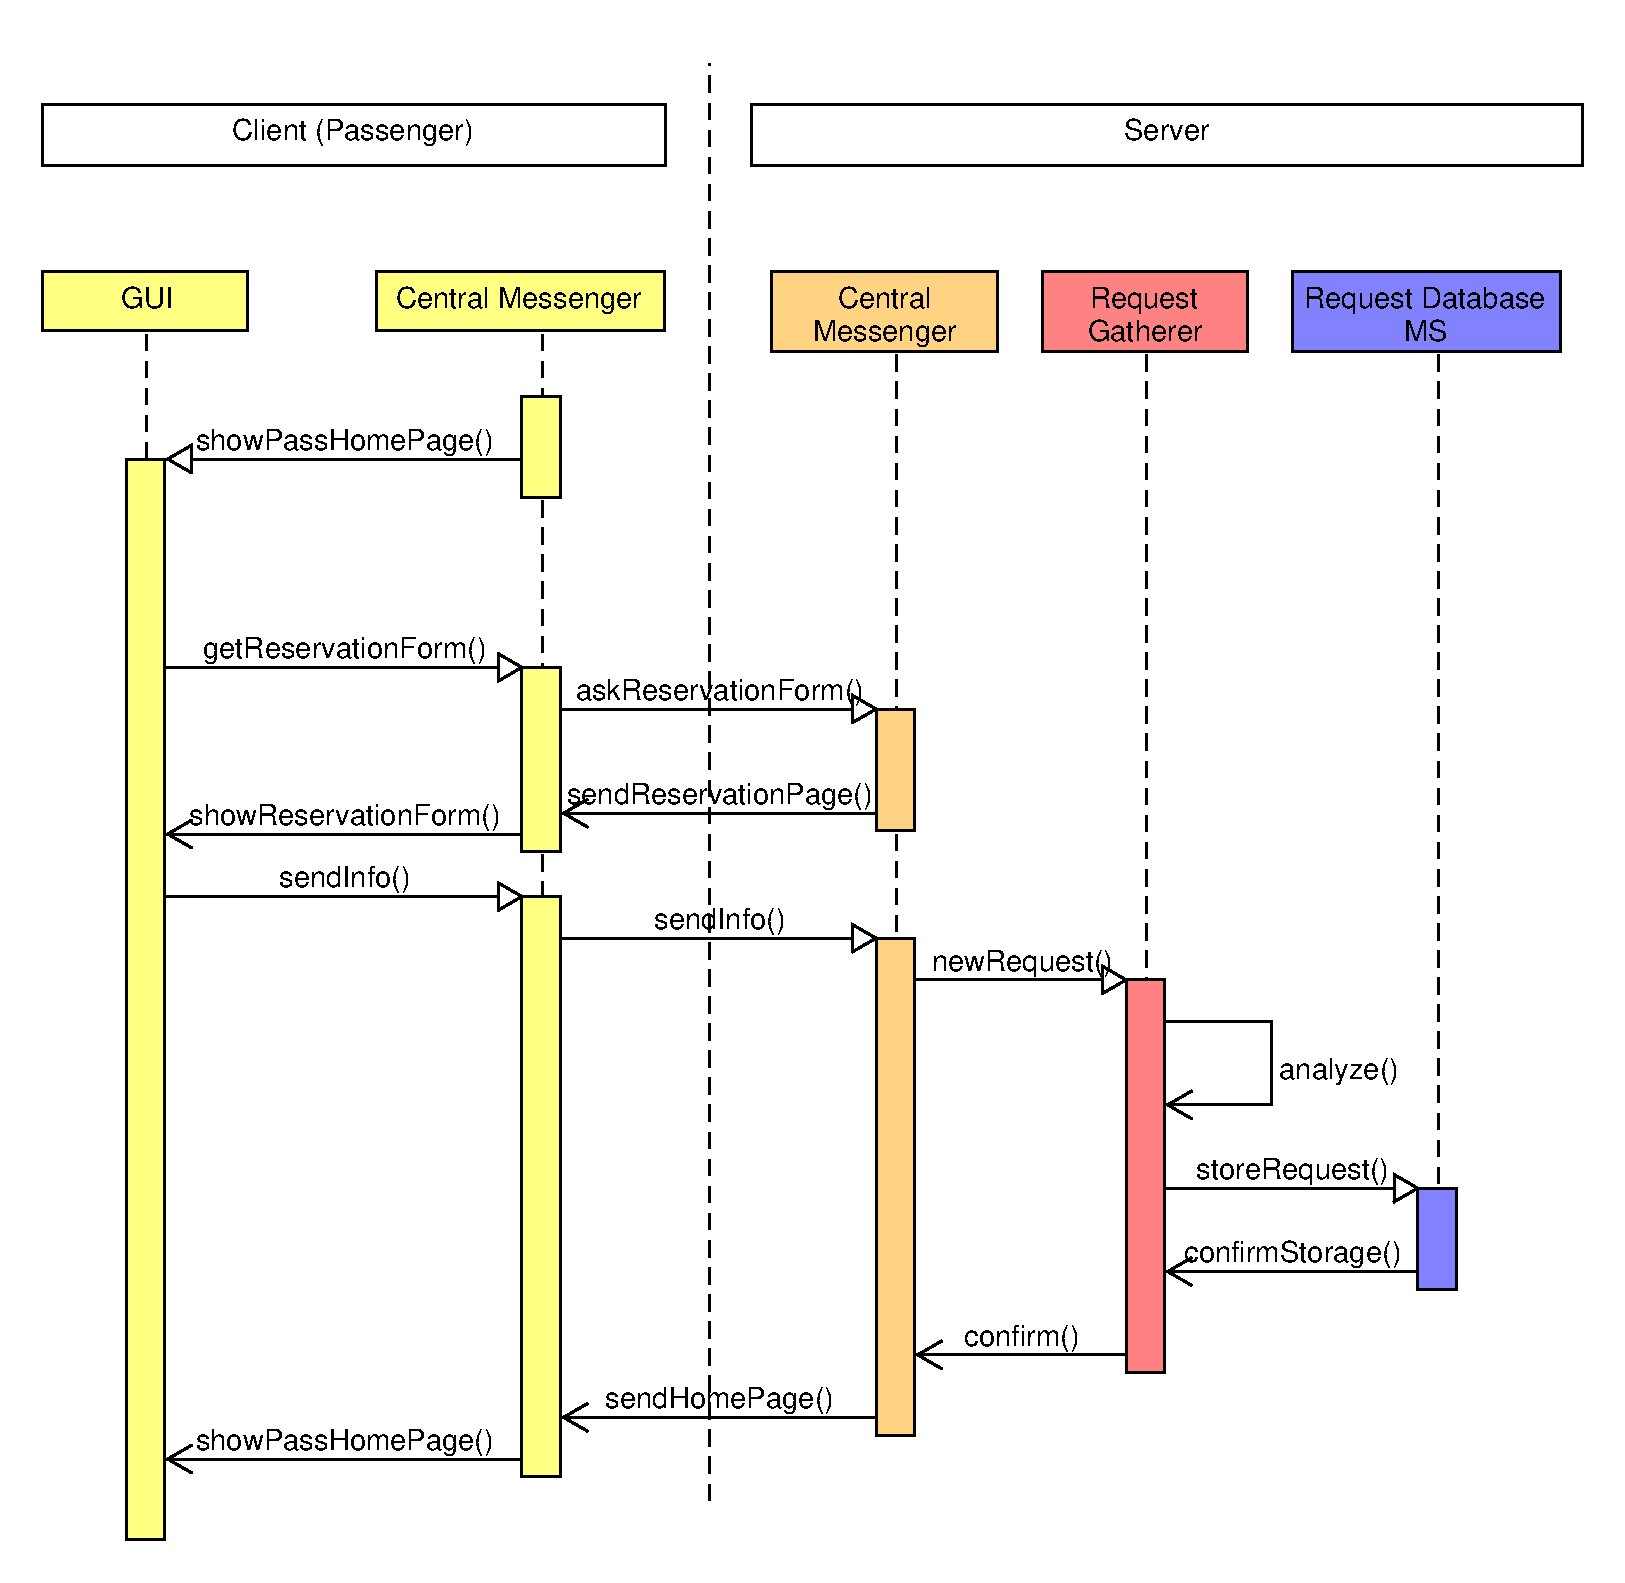
\includegraphics[width=\textwidth]{tex-images/sequence-1}
\caption{New reservation registration}
\end{figure}

\begin{figure}
\centering
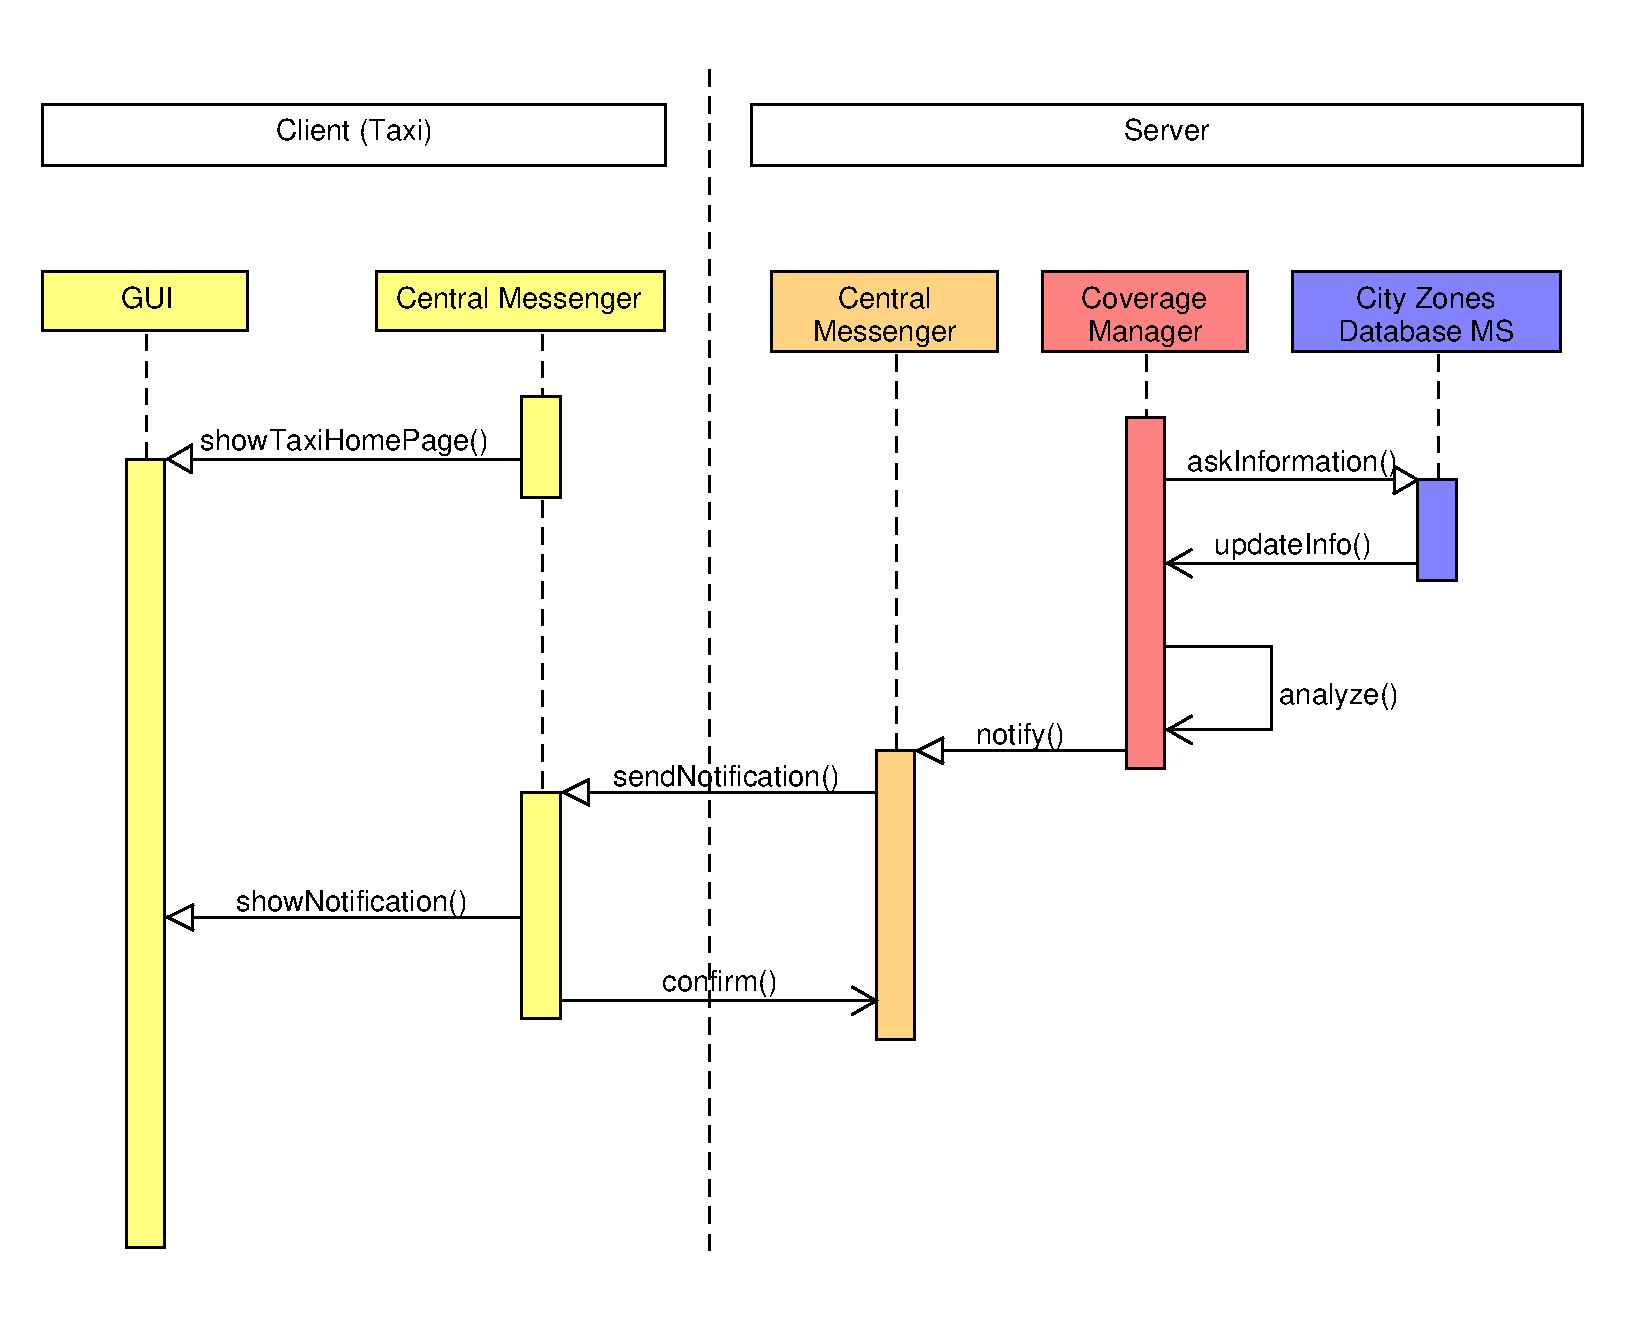
\includegraphics[width=\textwidth]{tex-images/sequence-2}
\caption{Coverage updates}
\end{figure}

\begin{figure}
\centering
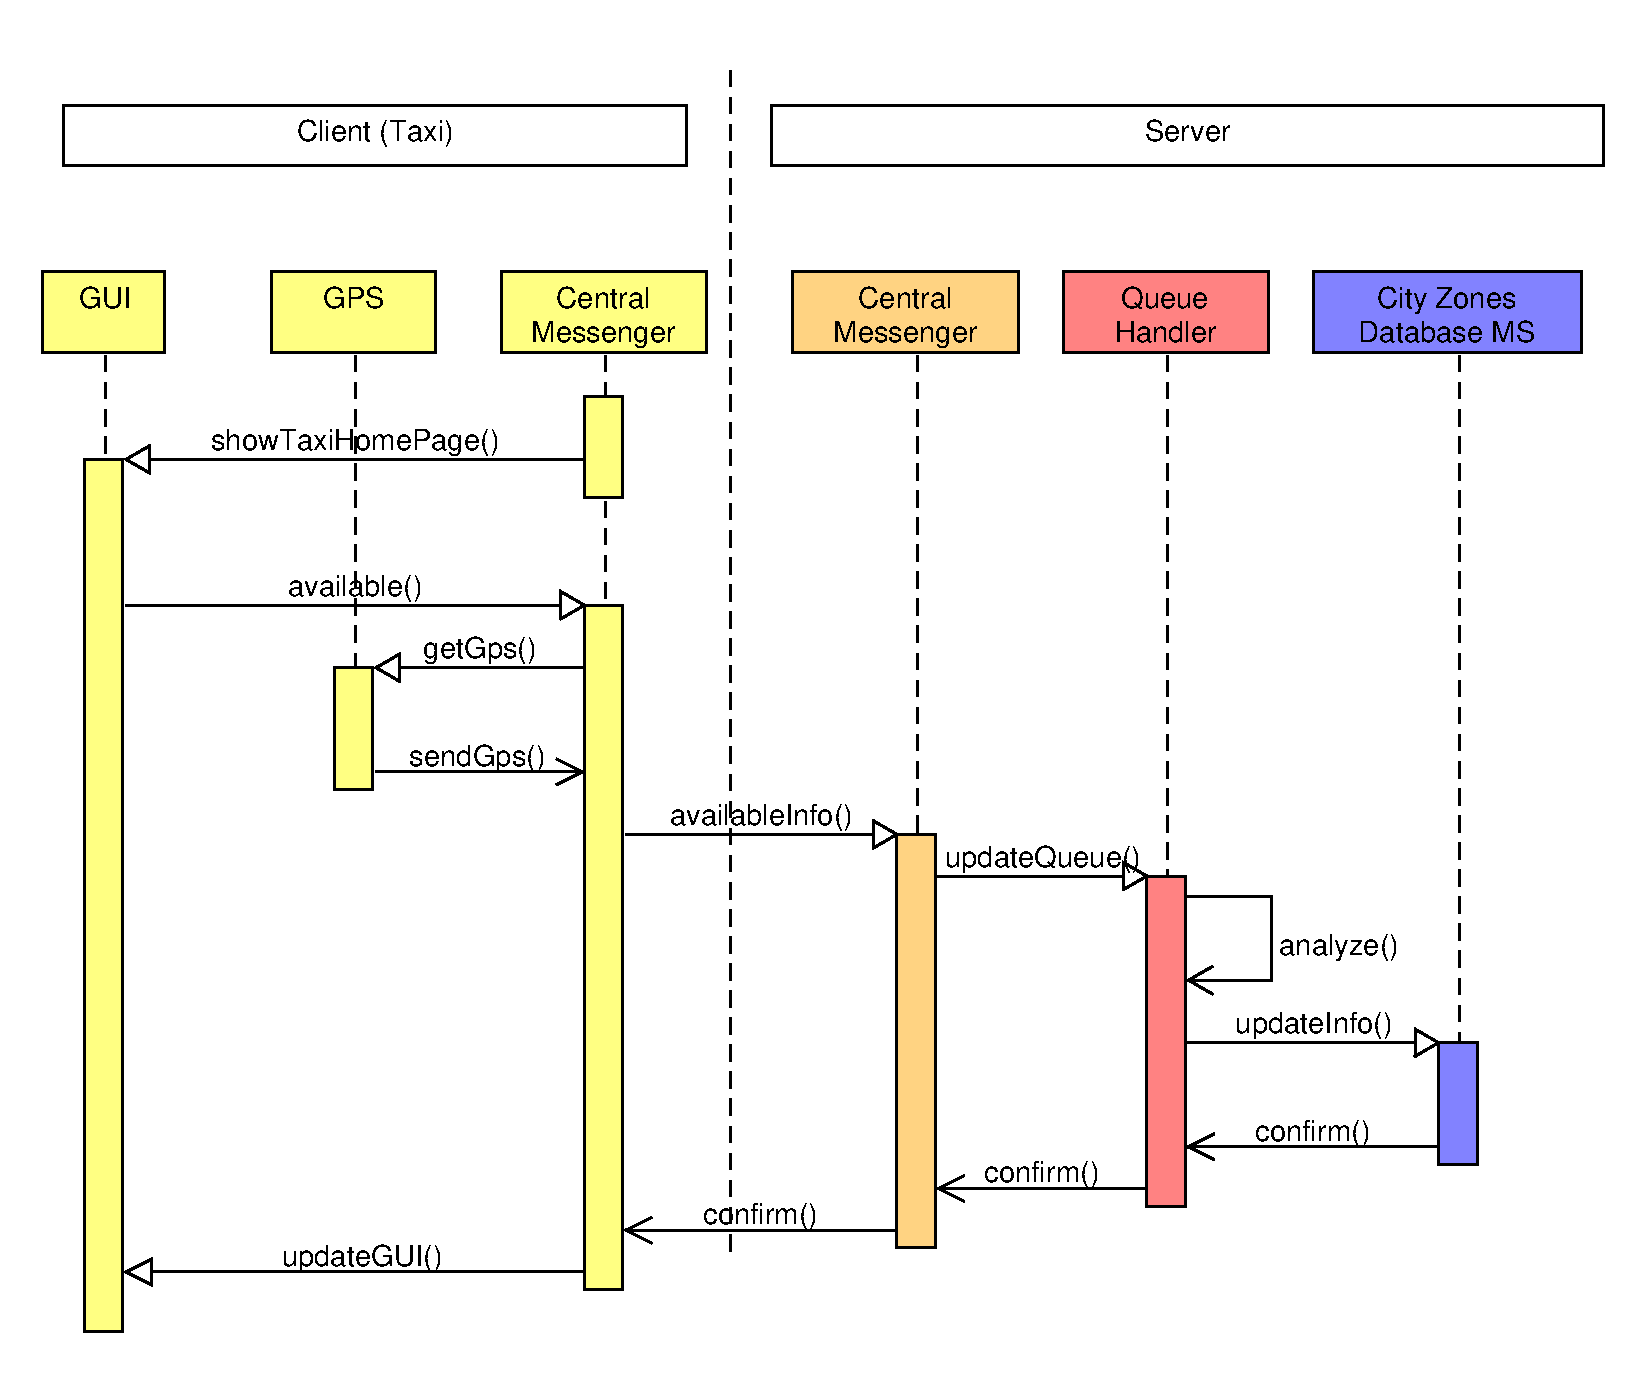
\includegraphics[width=\textwidth]{tex-images/sequence-3}
\caption{Taxi driver queues updates}
\end{figure}

\begin{figure}
\centering
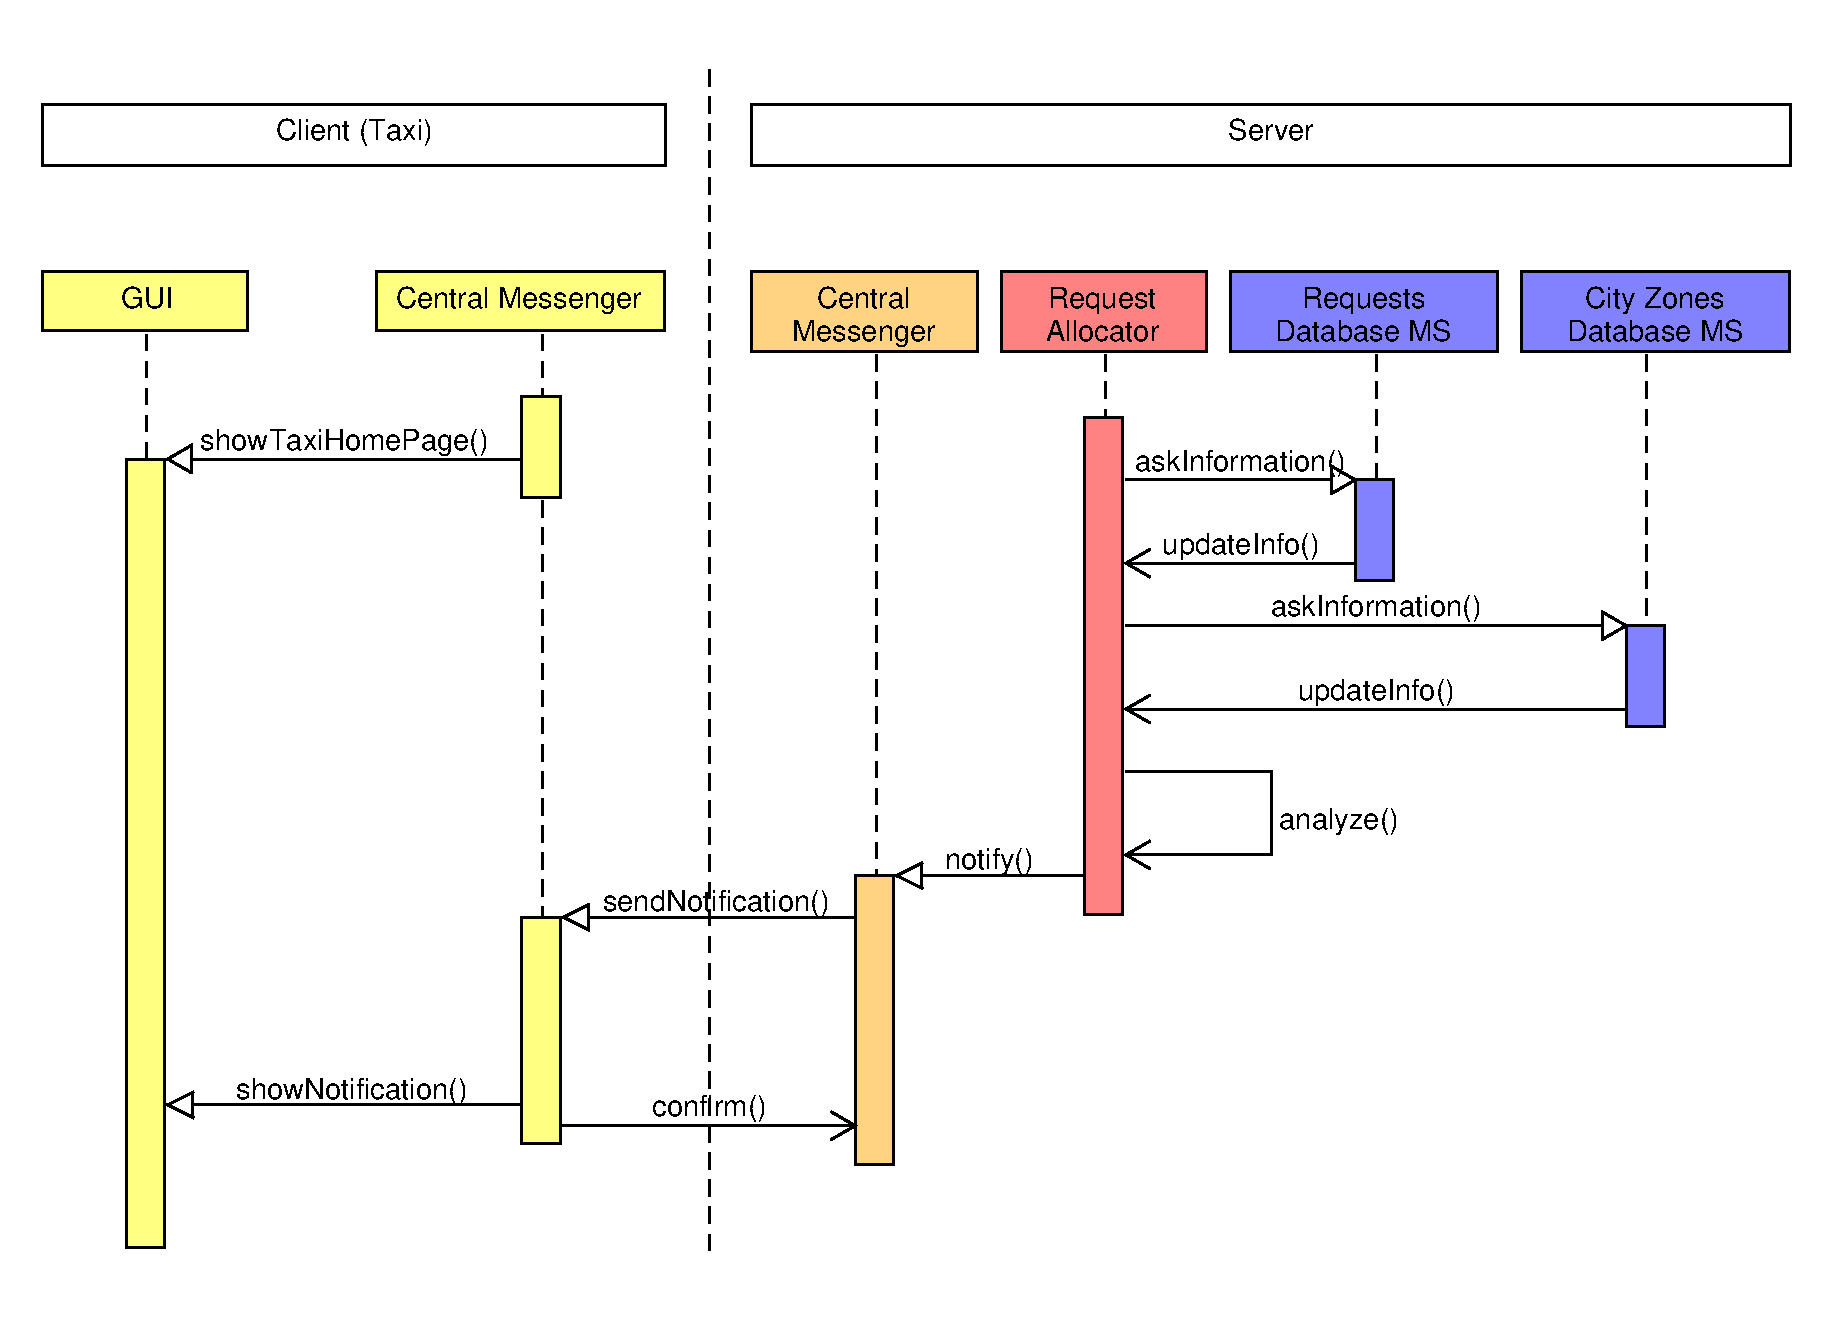
\includegraphics[width=\textwidth]{tex-images/sequence-4}
\caption{Reservation allocations}
\end{figure}

We have produced some run-time sequence diagrams of the main operations that can be made with the software, namely:
\begin{itemize}
\item Receive and register a new reservation;
\item Coverage cyclic checks and uptates;
\item Taxi driver queue updates;
\item Reservation allocations.
\end{itemize}

%%%%%%%%%%%%%%%%%%%%%%%%%%%%%%%%%%%%%%%%

\section{Component interfaces}
\begin{figure}
\centering
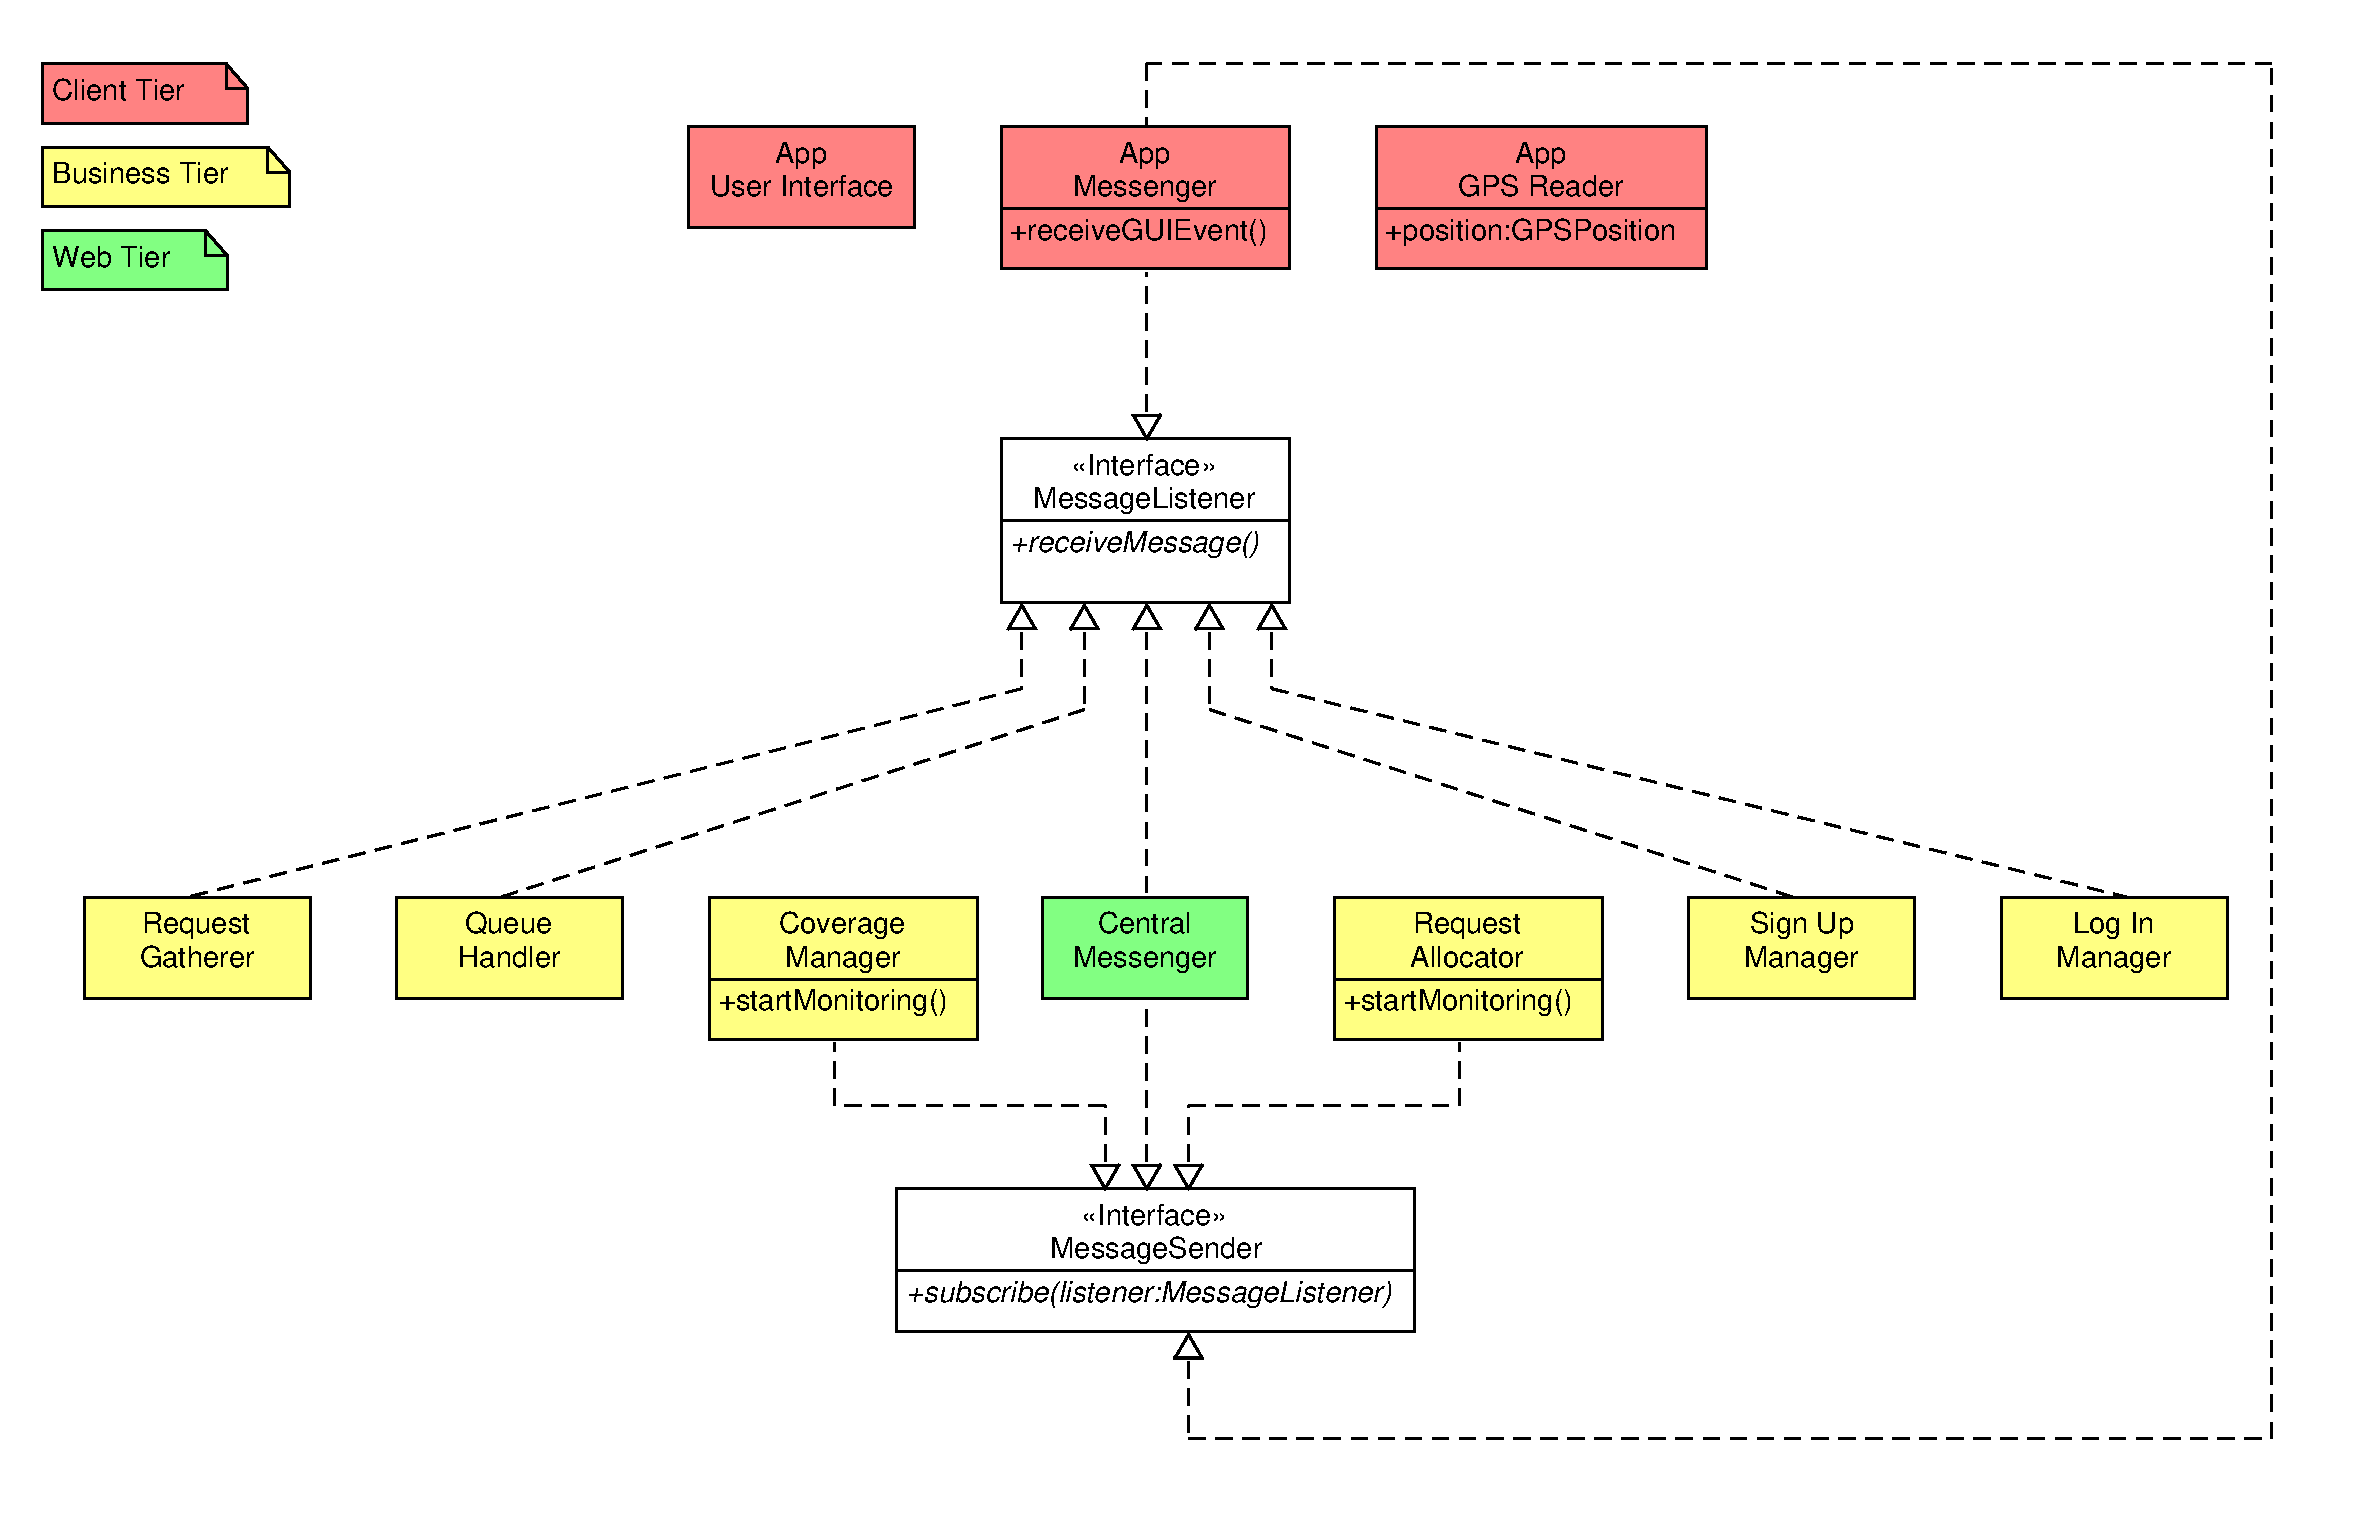
\includegraphics[width=\textwidth]{tex-images/interfaces}
\caption{Component interfaces}
\end{figure}

An Event-based style being used, components have little to no public interfaces to show to the outside world. Every information exchange taking place in the system, any order being given and received, everything is passed along as a \emph{message} event, to which each component, upon inspecting its contents, will react according to what it knows it needs done. As such, every representation of such interfaces is by definition barebone, but a diagram is included for the sake of clarity.

%%%%%%%%%%%%%%%%%%%%%%%%%%%%%%%%%%%%%%%%

\section{Architectural styles and patterns}
With regards to the general architecture, we found the problem at hand to be \emph{intrinsically} made to be solved by a client-server approach, and moreso we developed it in the particolar flavor of \emph{fat server} (since the application server runs the data tier, web tier, business tier) and \emph{thin client}. This architecture is exceedingly well supported and ready to be developed with JEE.

Additionally, we found most natural to design an event based architecture through an intense flow of messages among components. We choose this style because our components are very independent and in most of cases they interact asynchronously with each other.

%%%%%%%%%%%%%%%%%%%%%%%%%%%%%%%%%%%%%%%%

\section{Other design decisions}
We have paid particular attention in designing a very modular architecture favoured by having chosen a top-down approach. This disposition has been selected in order to facilitate future extensions.